\chapter{ROS Navigation} \label{ch:BaseWork}

%%\section{Introduction}
\section {ROS}
Creating software for robotic applications is not an easy task to do from scratch. It usually involves very complex code to achieve even the simplest applications due to the wide variety of hardware and data that robots rely on. \ac{ROS} fixes this issue by being a general purpose framework for robotics. Despite its name, it is not an operating system, it is more a kind of middleware, in other words it  handles communication between programs in a distributed system. You can either construct one program that does all the computation needed in your application or you can have sub programs with each one having a specific functionality, the latter is often preferred.

\ac{ROS} provides hardware abstraction, device drivers, tools for introspection, message-passing and more. Also it is open source which means we can use them for virtually any means which we deem necessary for the development of our application, for example adapting pre established code for a specific case. This greatly facilitates the entrance of new developers to learn and do research in this field.
\subsection{ROS architecture}
The \ac{ROS}  architecture is based on a peer to peer network between processes usually referred to as \textit{Computation Graph}. This structure is comprised by different concepts that we define bellow:
\begin{itemize}
\item \textbf{Nodes} - A node can be defined as a process or piece of software  that performs some type of computation. In \ac{ROS}, for a given application there are typically alot of nodes running in parallel that pass information between each other. For example  controlling the robot movement given the input image of a camera requires a node to act as a driver between the camera firmware and the ROS environment. Then there could be a node that processes the image further using ROS pre established software and finally given the processed information a different node will calculate the velocity of the robot and transmit them to the wheels of the robot. 
\item \textbf{Messages} - \ac{ROS} uses predefined data structures  called messages to interpret information. This makes it so \ac{ROS} tools to generate the appropriate source code in the selected language (C++ or phyton in this case). Each message can be broke down into more messages and so one and so forth until we arrive at the primitive data types of the given programming language. Nodes communicate by publishing or subscribing  to topics using this messages and in the end we get a fully alive system that performs some type of application we want. 
ROS predefined data type used to communicate between nodes.
\item \textbf{Topics} - Nodes can send messages by publishing to a topic or receive them by subscribing to a topic. For example a node can be subscribed a raw velocity message and then after some data processing publish a smoothed version of it into another topic.  
\item \textbf{Master} - Provides registration and naming for each node (helps nodes find each other). It is also responsible for organizing communication between nodes. Finnaly it also provides the \textbf{Parameter Server} (described bellow).
% V
\item \textbf{rosout} - This can be viewed as the ROS equivalent of stdout. This tool acts as a log reporting mechanism which is useful when debugging large amounts of code.
\item \textbf{Paramater Server} -In this server \ac{ROS} tracks different paramater values defined by the running application. It is useful for modifying different parameters dynamically without having to restart the application.
%X
\end{itemize}


%%REVER ISTO

Figure \ref{fig:rosgraph} gives a brief overview of how each of this concepts are put together and  generate the in ROS  computation system.

\begin{figure}[h] 
\centerline{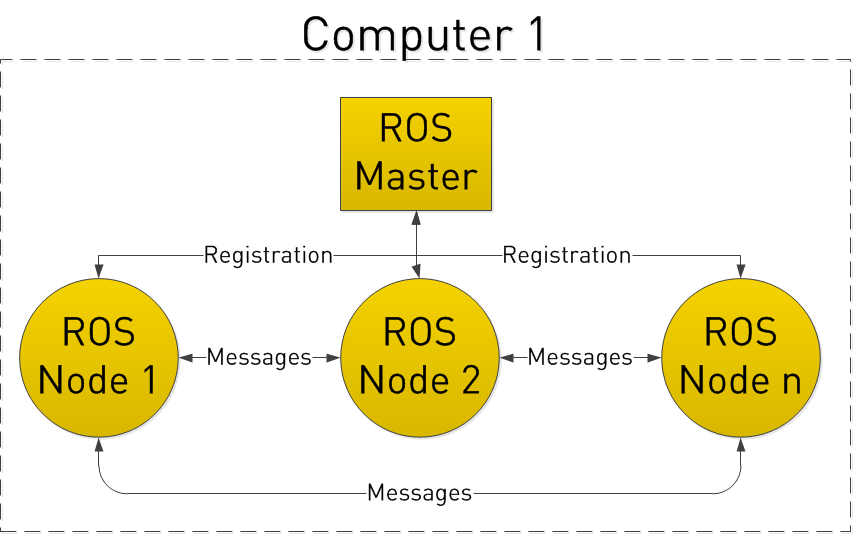
\includegraphics [width=0.8 \textwidth]{imgs/chapter3/rosgraph.png}}
\caption{ROS communication architecture overview \cite{rosbasics}}
\label{fig:rosgraph}
\end{figure}


%\section{Architecture Overview}\label{ch:requirements}
\section {Navigation Concepts}
There are four main problems associated with robotic autonomous navigation. They are Cognitive Mapping, Localization, Path Planning and Motion Control \cite{nav} as shown in Fig. \ref{fig:probNav} . 

\begin{figure}[h] 
\centerline{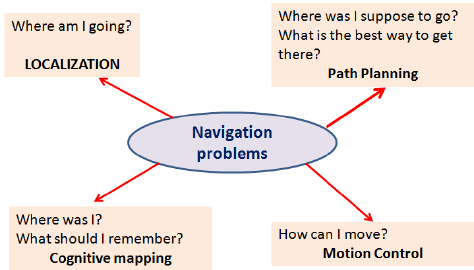
\includegraphics [width=0.8 \textwidth]{imgs/chapter3/probNAV.png}}
\caption{Problems regarding autonomous navigation \cite{rosbasics}}
\label{fig:probNav}
\end{figure}
Various algorithms have been developed over the years to combat this problems. 
%%Mapping

In regards to creating a suitable map,  \ac{ROS}  typically uses an improved version of  Rao-Blackwellized particle filters such as the ones described in \cite{grisetti2007improved}. This approach has proven to be an effective way to solve the \ac{SLAM} problem and will be used later on in this work to produce a valid map of our indoor environment.
%%Localization

With the grid map built we now need to estimate the robot's position in said map. 
An easy solution to this problem is relying on the robot's odometry information inferred by the robot's encoders and inertial sensors such as accelerometers and gyroscopes. This is called dead reckoning and is an easy and low cost solution for the localization problem. However since the sensor data is integrated over time, this leads to the accumulation of errors which make this approach not feasible for long navigation tasks. 
To fix this issue various algorithms were developed being the most popular ones based on particle filters. The \ac{AMCL} \cite{amclpaper} algorithm  is the standard choice in this case. It takes into account a group of particles, each one corresponding to a certain robot state (position and orientation in this case). As the robot moves the least probable states are filtered out and  the particles should over time converge on the actual position of the robot.  

Assuming the robot can localize itself on the map with a reasonable error we can start sending navigation goals to the robot. To reach the goal the robot must be able to find a path that optimizes the travel distance while avoiding obstacles. The outputted plan can vary depending on the algorithm used. This type of planning is often refereed as a global path planner that will be discussed further n in a later section.

After the optimal plan is computed the final step is to determine the best velocity command that will be sent to the base.  The ROS navigation system follows a similar approach to the one used in \cite{gerkey2008planning}. A set of velocities are simulated during a given set of time and the corresponding predicted trajectories are  computed. This subject is often referred to as local path planner methods that will be further detailed bellow.
\section{Path Planning and Motion Control}
 Obstacle avoidance is a major subject in robotics, failure in this systems may result in crashes that have catastrophic consequences such as hardware being badly damaged or being completely nonfunctional. This problem is usually separated into two categories local path planning and global path planning \cite{foxdwa}. 
 Global methods assume the environment is completely known a priori and can therefore compute an optimal safe path  around static obstacles using a variety of different strategies. This models prove to be very reliable for static environments. However this models are usually computational expensive which lead to very slow update times. For fast changing environments such as is in the case for highly populated indoor scenarios they prove to be insufficient. 
 To improve the quality of navigation capabilities, local path planning techniques are added to improve the responsiveness of the robot. This techniques have a much faster update time  since they use a smaller version of the world around them. However this type of approaches have trouble with local minimum cases where the robot gets stuck (for example the U-shape case).
\subsection{Global Methods}
Path planning is crucial for the robot to handle safe trajectory around obstacles. In this work the information regarding this obstacles is based on a grid map built by \ac{SLAM} and new observations retrieved by the robot's sensors.  Planning an optimal safe path can be done using a wide variety of methods like Visibility Graphs, Generalized Voroin Diagram, and \ac{PRM} \cite{globalmethods}. However for in this work we will use the \ac{PRM} method. This method samples its environment and creates a occupancy graph. Then by inserting the initial position and the goal position the path can be computed using dijaktra or A* or Rapidly exploring Random Trees search algorithms . However, the \ac{ROS} navigation packages only use the first two so  we will only focus on this ones.


\subsubsection{Dijaktra algorithm}
Assuming we have an occupancy map we can now start to explain how does a robot compute the shortest path between the starting position and the end goal. Edsgar W. Dijkstra proposed an algorithm that solves this problem for a number of nodes, in our case we have cells on an occupancy grid map. Assuming with each cell costs the same then the shortest path can be calculated doing the following algorithm described in Figure \ref{fig:dalg}. 
\begin{figure}[h] 
\centerline{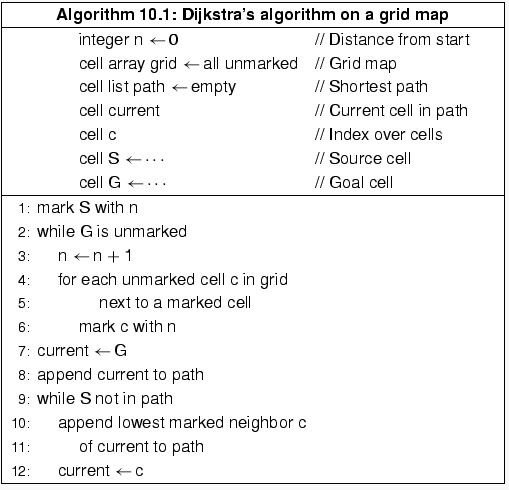
\includegraphics [width=0.7 \textwidth]{imgs/chapter5/Dalg.png}}
\caption{(taken form \cite{Ben-Ari2018})}
\label{fig:dalg}
\end{figure}
Each cell is numbered with the number of steps it needs to get to the starting position. This continues until we reach the goal cell and we get the minimum path to reach it. However if we have a map with cells that have variable cost in the algorithm above we do not iterate $n$ with plus one, but with the cell cost. This makes it so for this case that  shortest path geometrically may not be the shortest path when the costs are taken into account.

\subsubsection{A* algorithm}
In the previous case we search for cells in all directions, however there is a more efficient way of doing it by adding more information. The A* algorithm takes into account an extra \textit{heuristic function} to that gives a preferred direction for the search. Not only does it take into account the cell cost but another value that corresponds to a given direction to be doing in  the search. The function can be shown as:
\begin{equation}
    f(x,y)=g(x,y) + h(x,y)
\end{equation}
\subsection{Local Methods}
In contrast to global path planning in where a large portion of the environment is generally assumed to be true, local methods take in to account a partial world view for the motion planning capabilities. In other words, local path planning determines the motion of the robot taking into account the global plan provided by the global methods described earlier.
The most popular of this type of methods are \cite{inbookdwa}:
%cite this
\begin{itemize}
    \item \ac{DWA} \cite{foxdwa}
    \item Trajectory Rollout  \cite{gerkey2008planning}
    \item Elastic Band \cite{siegwart2011introduction}
    \item Timed elastic band \cite{rosmann2013efficient}
    \item Tentacles Clothoid \cite{alia2015local}
    \item \ac{VFH}+ \cite{siegwart2011introduction}
\end{itemize}
For our case study we will only explore the first two that are already integrated in ROS.
\subsubsection*{\ac{DWA} planner}
The Trajectory Rollout  the most standard approach when it comes to local path planning in \ac{ROS}. It outputs  rotational and translational velocity by generating multiple trajectories for different types of velocity sample search space and choosing the best one. The algorithm goes as follows \cite{inbookdwa}:
\begin{itemize}
    \item Start with a set of velocities pairs $\{R_{vR_x},R_{ \omega_z} \}$ that are obtainable by the robot.
    \item Genarate in the form of arcs the projected trajectories obtained using the previous velocity sample space.
    \item Dismiss velocities that result in the robot colliding with an object in a given time frame. With this we are left of a subset of admissible velocities $V_a=R_{vR_a},R_{ \omega_a}$ in which:
    \begin{equation}
         V_a=R_{vR_a},R_{ \omega_a} \iff \begin{cases}
    R_{vR_x} & 	\leq \sqrt{2*dist(R_{vR_x},R_{ \omega_z})*R_{\dot{v}_{xb}}}.\\
    R_{ \omega_z}  &  	\leq \sqrt{2*dist(R_{vR_x},R_{ \omega_z})*R_{\dot{\omega}_{zb}}}.
  \end{cases}
    \end{equation}
    Where $R_{\dot{v}_{xb}}$ and $R_{\dot{\omega}_{zb}}$ are the braking accelerations of the robot and $dist$ the distance to the closest obstacle on the trajectory.
    
    
    \item Dismiss velocities that don't respect the robot's acceleration limits in a given simulated time frame. With this we are left with a subset of velocities called dynamic window $V_d=R_{vR_d},R_{ \omega_d}$  in which:
    \begin{equation}
         V_d=R_{vR_d},R_{ \omega_d} \iff \begin{cases}
    R_{vR_x} & 	\in [R_{v_a}-R_{\dot{vR}_{x}}*t,R_{v_a} + R_{\dot{vR}_{x}}*t].\\
    R_{\omega_z} & 	\in [R_{ \omega_a}-R_{\dot{\omega}_{z}}*t,R_{\omega_a}+R_{\dot{\omega}_{z}}*t].\\
  \end{cases}
    \end{equation}
    \item Finally we choose  the most optimal trajectory and in consequence velocity pair taking into account a given objective cost function.
    The cost function used to evaluate a trajectory in the \ac{ROS} navigation stack local planners is given by:
    \begin{align*}
            \textbf{cost} = &
       \texttt{pdist\_scale} * \textbf{path\_dist}
       + \texttt{gdist\_scale} * \textbf{goal\_dist}\\
       &+\texttt{occdist\_scale} * \textbf{maxobscost} 
    \end{align*}
    
    Where \textbf{path\_dist} is the distance from the endpoint of the trajectory to the global path in map cells, \textbf{goal\_dist} is the distance from the endpoint of the trajectory to the local goal in map cells, and \textbf{maxobscost} is equal to the \textbf{maximum obstacle cost} (given by the local costmap) of all the points along the trajectory.
    \end{itemize}
\section {ROS Navigation stack}
The ROS navigation stack is a set of software packages that properly combined can get a robot to navigate autonomously.
Figure \ref{fig:plans} shows an example of \textbf{turtlebot2} using the navigation stack to drive autonomously.
\begin{figure}[!htb]
    \centering
    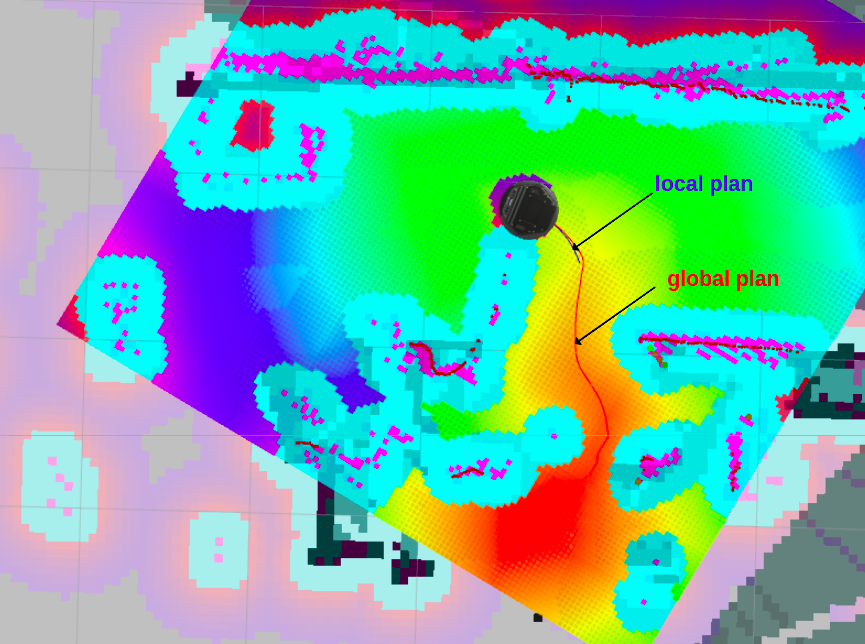
\includegraphics[width=\linewidth]{imgs/chapter3/nav.png}
    \caption{Rviz displaying the ros navigation stack components while \textbf{turtlebot2} is navigating.}
    \label{fig:plans}
\end{figure}

\subsection{Requirements}
 Before running the \ac{ROS} navigation stack we first need to properly setup the robot that meet its requirements.
\subsubsection{Transform Configuration}
The Navigation stack requires that the relationships between the different frames must be published in \textbf{tf} or \textbf{tf\_static} topic. This makes it so the robot perceives what is around him correctly.
Figure \ref{fig:tf} shows all the frames and their transforms with each other for \textbf{turtlebot2}. However the main transforms that need to be correct are between the sensors and the base link frame.
\begin{figure}[!htb]
    \centering
    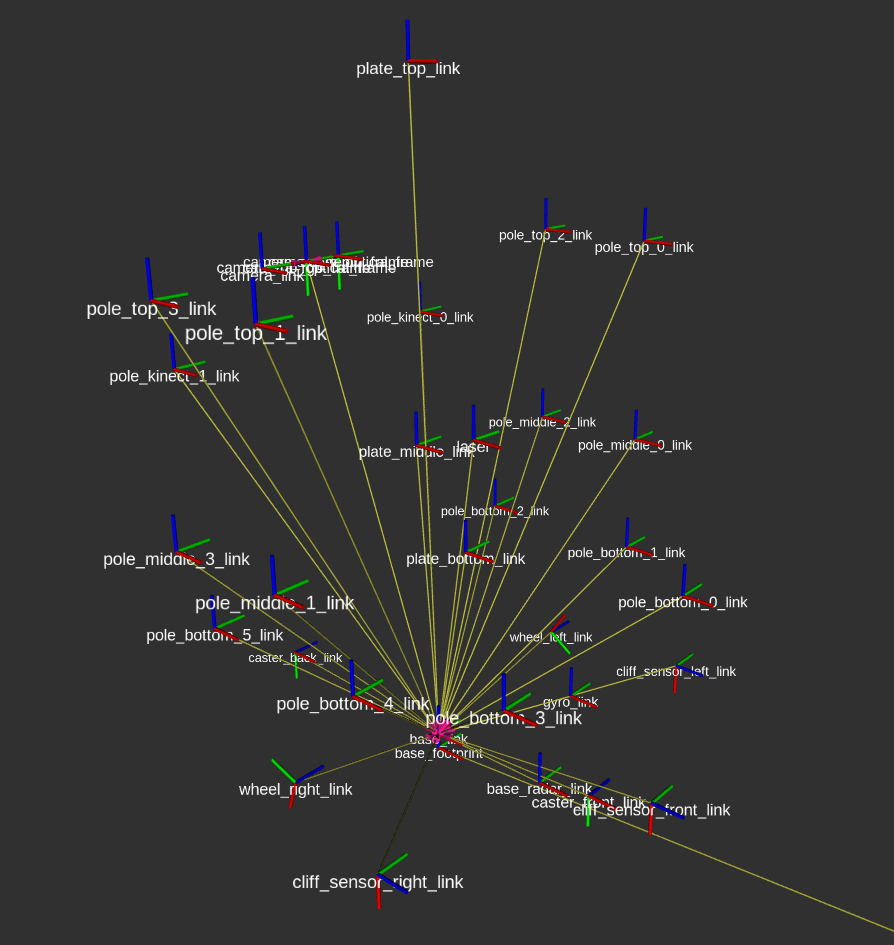
\includegraphics[scale=0.4]{imgs/chapter3/tf.png}
    \caption{Transform relationships in our robot}
    \label{fig:tf}
\end{figure}

\subsubsection{Sensor sources}
To avoid obstacles we need some type of sensors that can detect them. Before running the stack we need to make sure they are publishing this information.
In our case we will use both the \textbf{\ac{FMCW}} \textbf{\ac{radar}} (PointCloud2) and the \textbf{\ac{LiDAR}} (LaserScan) as our observation sources.
Figure \ref{fig:sensors} shows an example of the published data from both in rviz.
\begin{figure}[!htb]
    \centering
    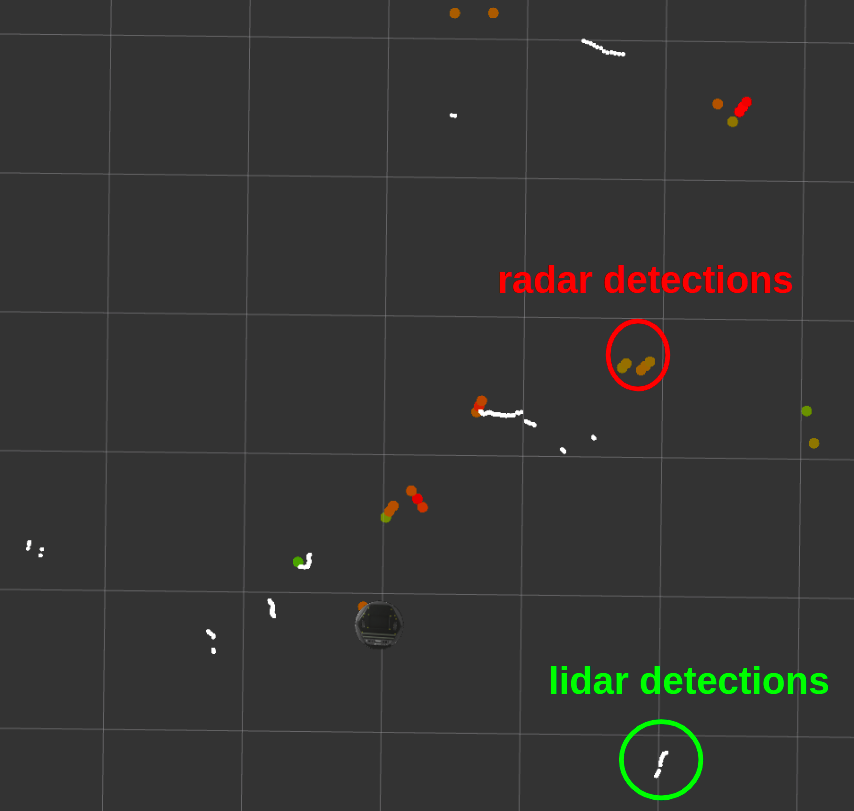
\includegraphics[scale=0.5]{imgs/chapter3/sensors2.png}
    \caption{Obstacle defections by both radar and lidar}
    \label{fig:sensors}
\end{figure}
\subsubsection{Odometry}
We need to localize the robot in some way to correctly navigate. Therefore we require a topic that publishes odometry information.
\subsubsection{Base Controller}
This node will subscribe to the velocity message outputted by the navigation stack and convert them into the appropriate motor commands to send to the mobile base that will actually make the robot move.
%%GARBAGE
\subsubsection{Mapping}
This part is not mandatory but it helps to have a some sort of map being published to use as a global reference for the robot. It is used by \texttt{amcl} to correctly localize the robot and to mark previously detected lethal obstacles when the map was built. Fig. \ref{fig:map} shows an example of a map that might be used by the ROS navigation stack.
\begin{figure}[!htb]
    \centering
    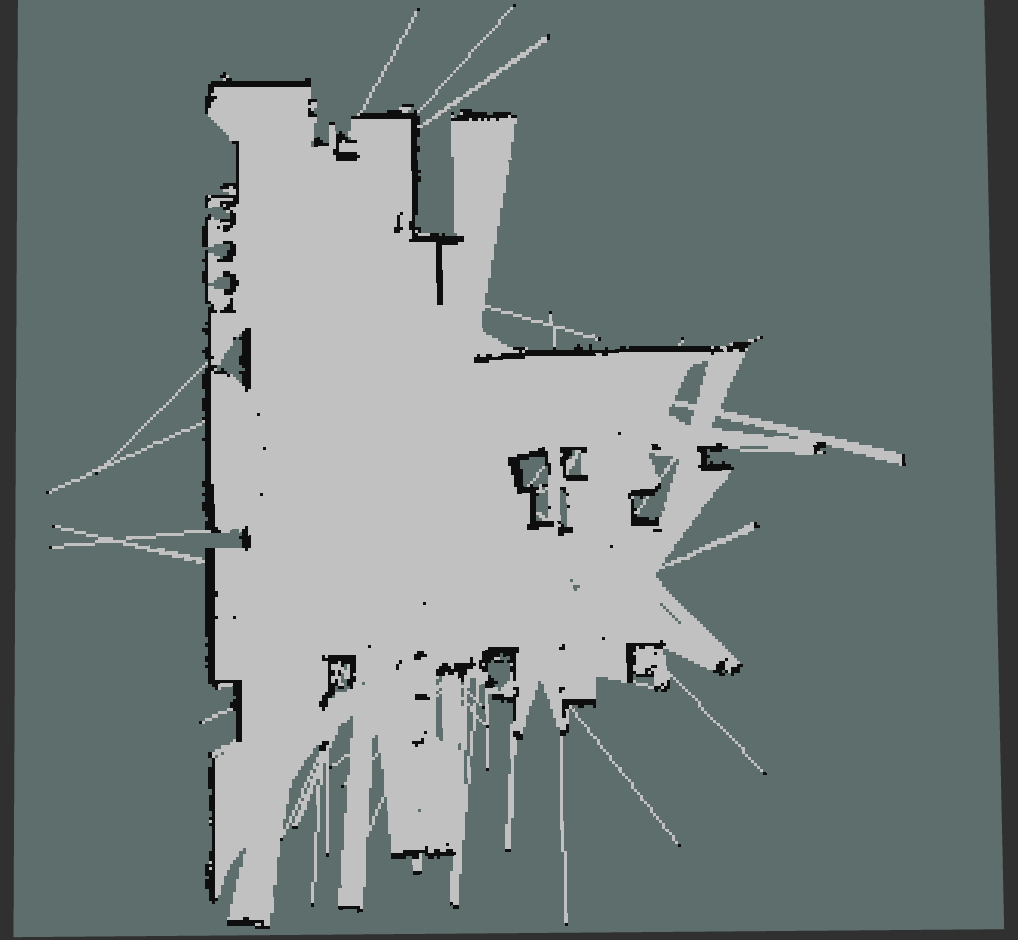
\includegraphics[scale=0.4]{imgs/chapter3/map2.png}
    \caption{Example of a map created in the IRIS laboratory}
    \label{fig:map}
\end{figure}
If the setup is done correctly we can now run the navigation stack.
\subsection{Navigation Stack components}
%%STUFF
Now that we have all the things we need for navigation we need an entity that actually processes all this information in an intelligent way to determine the best velocity command for the robot. This is done by the \texttt{move\_base } node and its peripherals.
Figure \ref{fig:nav_stack} shows an overview of the different components of the navigation stack \cite{movebase}.
\begin{figure}[!htb]
    \centering
    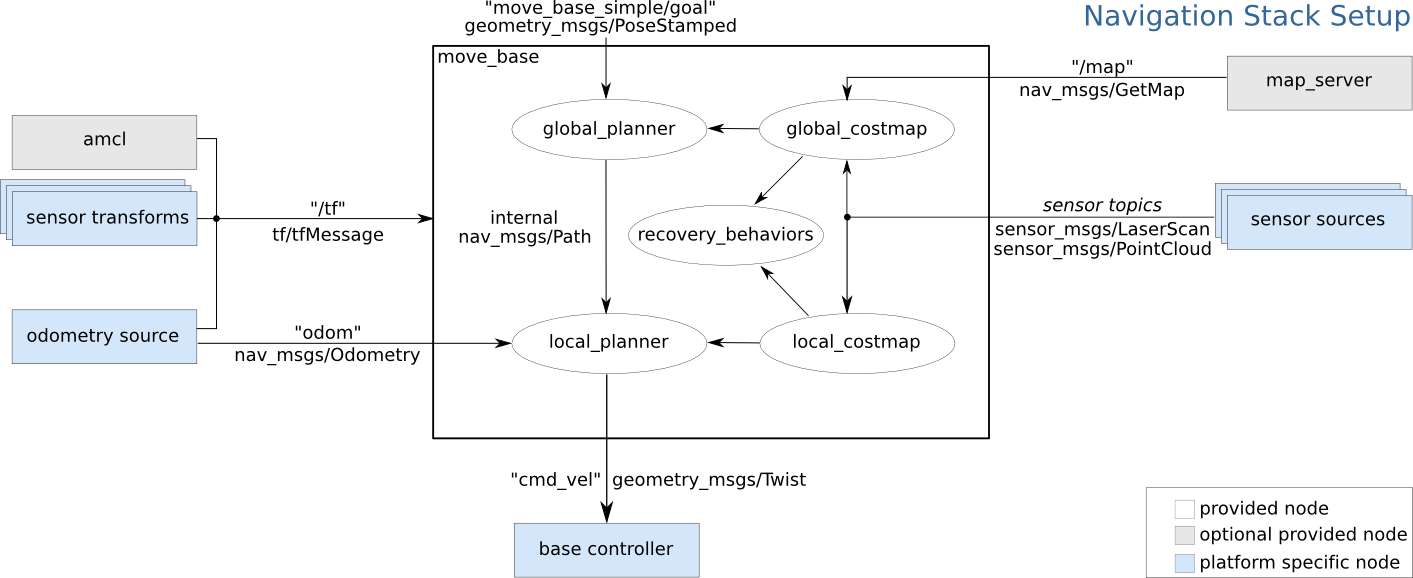
\includegraphics[width=\linewidth]{imgs/chapter3/navstack.png}
    \caption{Navigation stack block diagram}
    \label{fig:nav_stack}
\end{figure}
\subsubsection{Move Base}

The move base node base links together a global and local planner as well as a local and global costmap to achieve the end goal provided by an action server. It also loads a set of determined recovery behaviors if the planners fail to produce a valid path. 

The global and local planners are plugins specified by the user. This choice will affect the behavior of the robot depending on the planners architecture and parameters. In this work it will be used \textbf{navfn} as our global planner and \textbf{TrajectoryPlannerROS} as our local planner.

\subsubsection{Global Planner}
 
The job of this component is to produce the best trajectory for a robot to take with limited amount of information given by the global costmap.
This plan can be updated when the robot gets stuck or by a user specific frequency. The algorithms used to get this path are usually \textbf{djakarta} or \textbf{A*} that are described in the previous section.

\subsubsection{Local Planner}
The local planner takes into account the trajectory given by the global planner and tries to compute velocity commands that follow it. However the path given may be to close to an obstacle detected and in order to avoid it we must deviate from the plan given to avoid collision. The function of the local planner is to avoid dynamic obstacles that appear while still trying to follow the global plan and goal. This type of local planner is usually \textbf{TrajectoryPlannerROS} or \textbf{DWAPlanner} that follow the explanation in the previous sections.
\subsubsection{Local and Global Costmap}
The global and local costmap share the same class, the  \texttt{Costmap2DROS}. This class consists of a layered costmap that takes into account various layers defined by the user.

\subsubsection*{Available Layers}
\begin{itemize}
    \item \textbf{Obstacle Layer} - Marks objects retrieved from our sensor sources with lethal value. It also raytraces observations to clear out space.
    %Does more stuff
    \item \textbf{Inflation Layer} - Inflates the detected obstacles taking into account the robot radius and inflation radius. The closer the cells are from a lethal obstacle the more value they will have.
    %%....(needs explanation)
    \item \textbf{Static Layer} - Retrieves static information from the \textbf{/map} topic and marks them has lethal objects (Typically only used in global costmap).
\end{itemize}





